\begin{frame}{Object Detection}
  \begin{figure}
    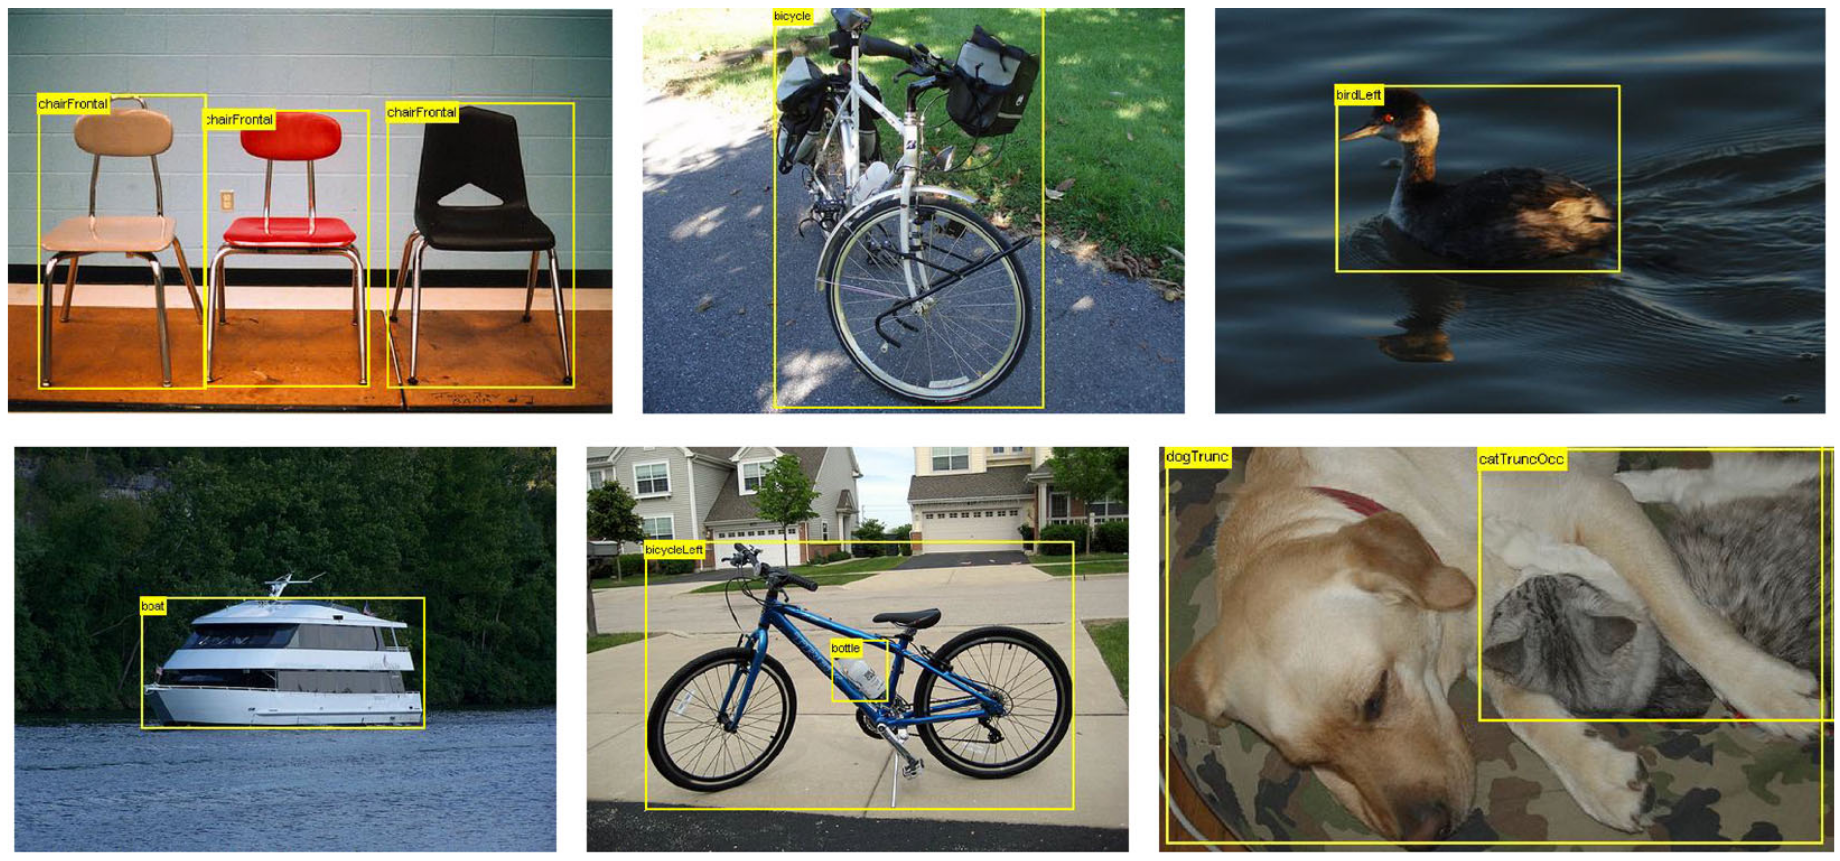
\includegraphics[width=0.9\textwidth]{detection_pascal_voc}
  \end{figure}

  \note{
    \begin{itemize}
      \item Image from The PASCAL Visual Object Classes Challenge: A Retrospective, Everingham et al, IJCV 2014
    \end{itemize}
  }
\end{frame}


\begin{frame}{Dataset: PASCAL Visual Object Classes}
  \begin{columns}
    \begin{column}{0.48\textwidth}
      \begin{figure}
        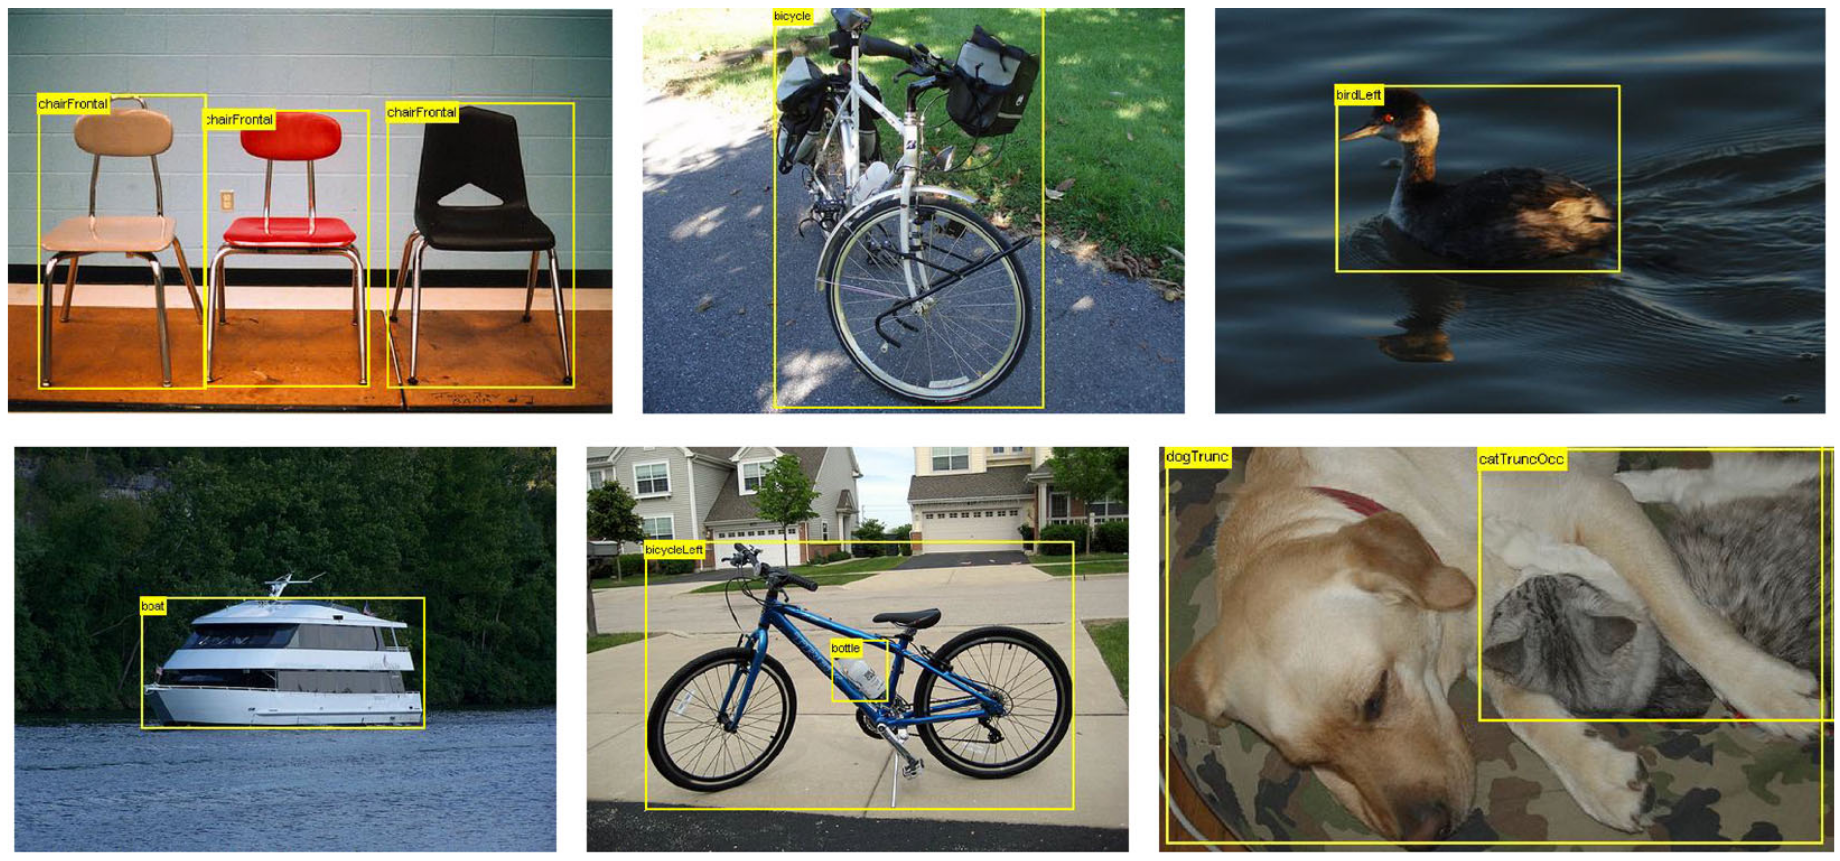
\includegraphics[width=0.9\textwidth]{detection_pascal_voc}
      \end{figure}
    \end{column}
    \begin{column}{0.48\textwidth}
    \begin{itemize}
      \item 20 classes
      \item 11k annotated images
      \item 27k annotated objects
    \end{itemize}

    \end{column}
  \end{columns}

  \note{
    \begin{itemize}
      \item Pascal VOC (DPM 33.6\%)
    \end{itemize}
  }
\end{frame}


\begin{frame}{Intersection over Union}
  Detection is correct if
  $$ intersection/union > threshold$$

  \begin{figure}
    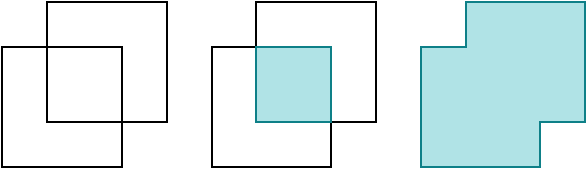
\includegraphics[width=0.9\textwidth]{iou}
  \end{figure}
  \note{
    \begin{itemize}
      \item Default threshold was 0.5 for a long time but is now often higher.
    \end{itemize}
  }
\end{frame}


\begin{frame}{Recall and Precision}
  \begin{align*}
    precision &= \nicefrac{\#(correct~detections)}{\#(all~detections)}\\
    recall &= \nicefrac{\#(correct~detections)}{\#(all~objects)} \\
  \end{align*}
      Average Precision: area under PR curve for specific class\\
      mean Average Precision: AP averaged over all classes
  \begin{figure}
    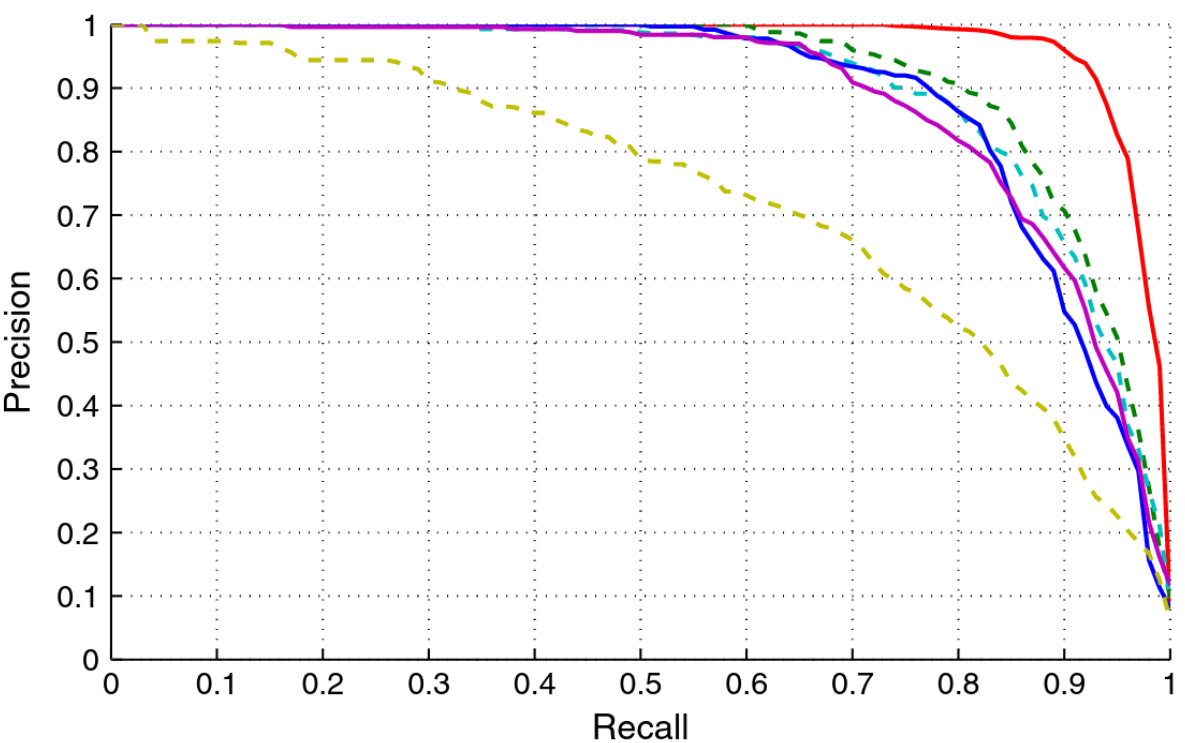
\includegraphics[width=0.5\textwidth]{precision_recall}
  \end{figure}

  \note{
    \begin{itemize}
      \item Image from The PASCAL Visual Object Classes Challenge: A Retrospective, Everingham et al, IJCV 2014
    \end{itemize}
  }
\end{frame}


\begin{frame}{Object Detection: output dimensionality?}
  \begin{figure}
    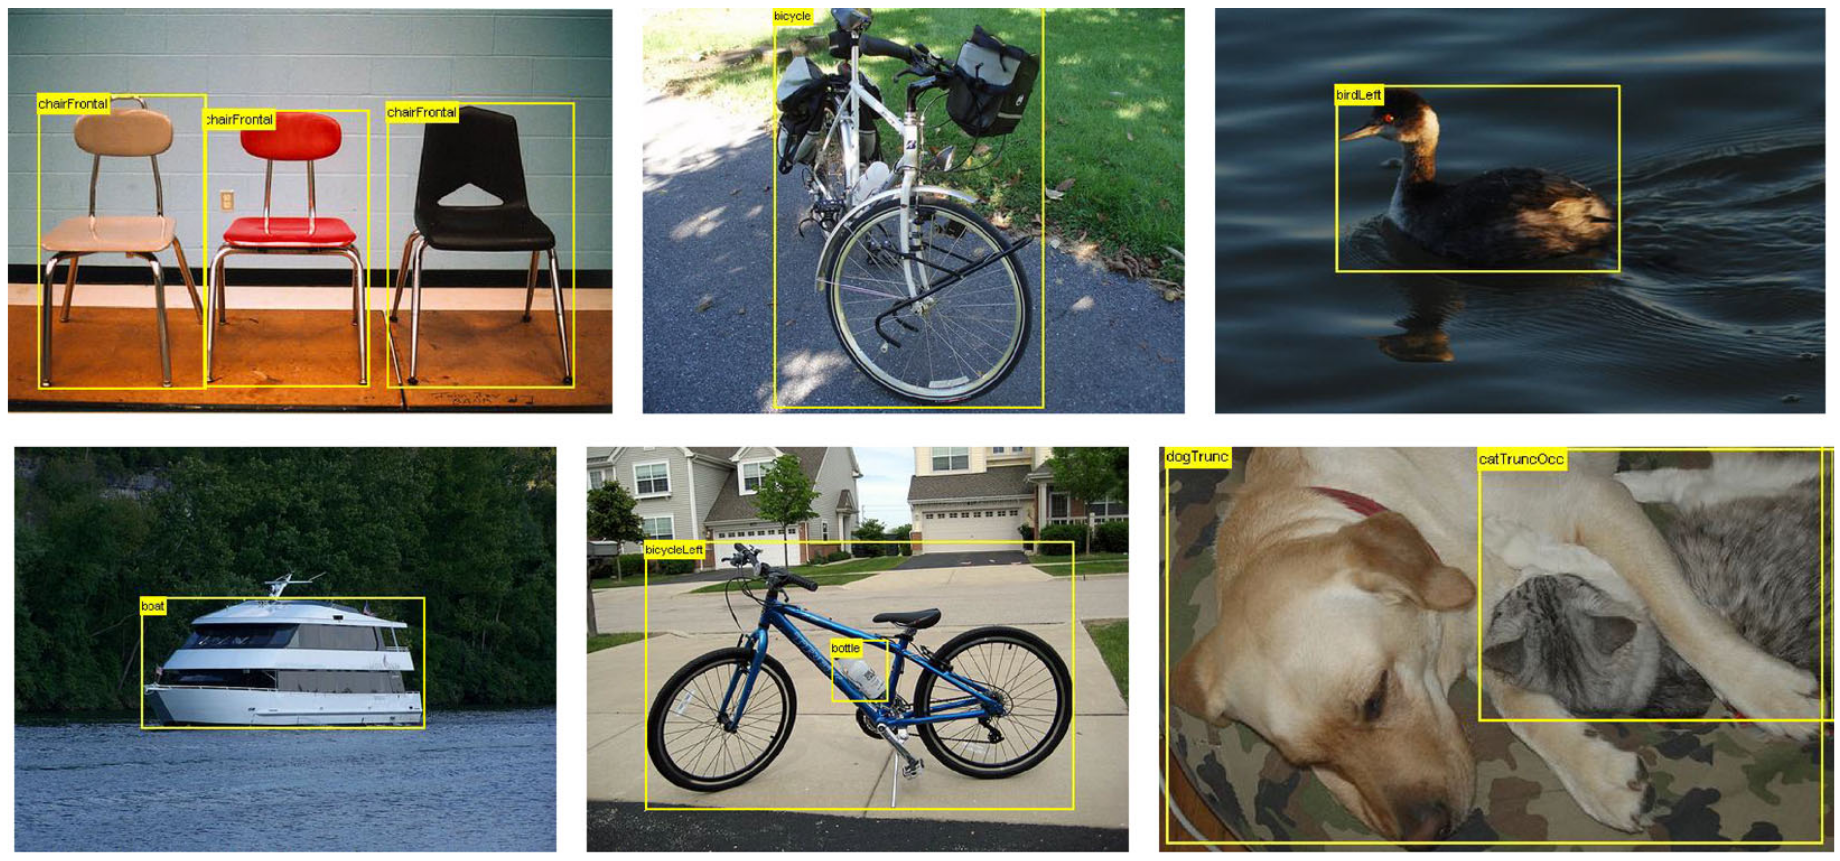
\includegraphics[width=0.9\textwidth]{detection_pascal_voc}
  \end{figure}

  \note{
    \begin{itemize}
      \item How would the head of this network look like?
      \item Image from The PASCAL Visual Object Classes Challenge: A Retrospective, Everingham et al, IJCV 2014
    \end{itemize}
  }
\end{frame}


\begin{frame}{R-CNN}
  \begin{figure}
    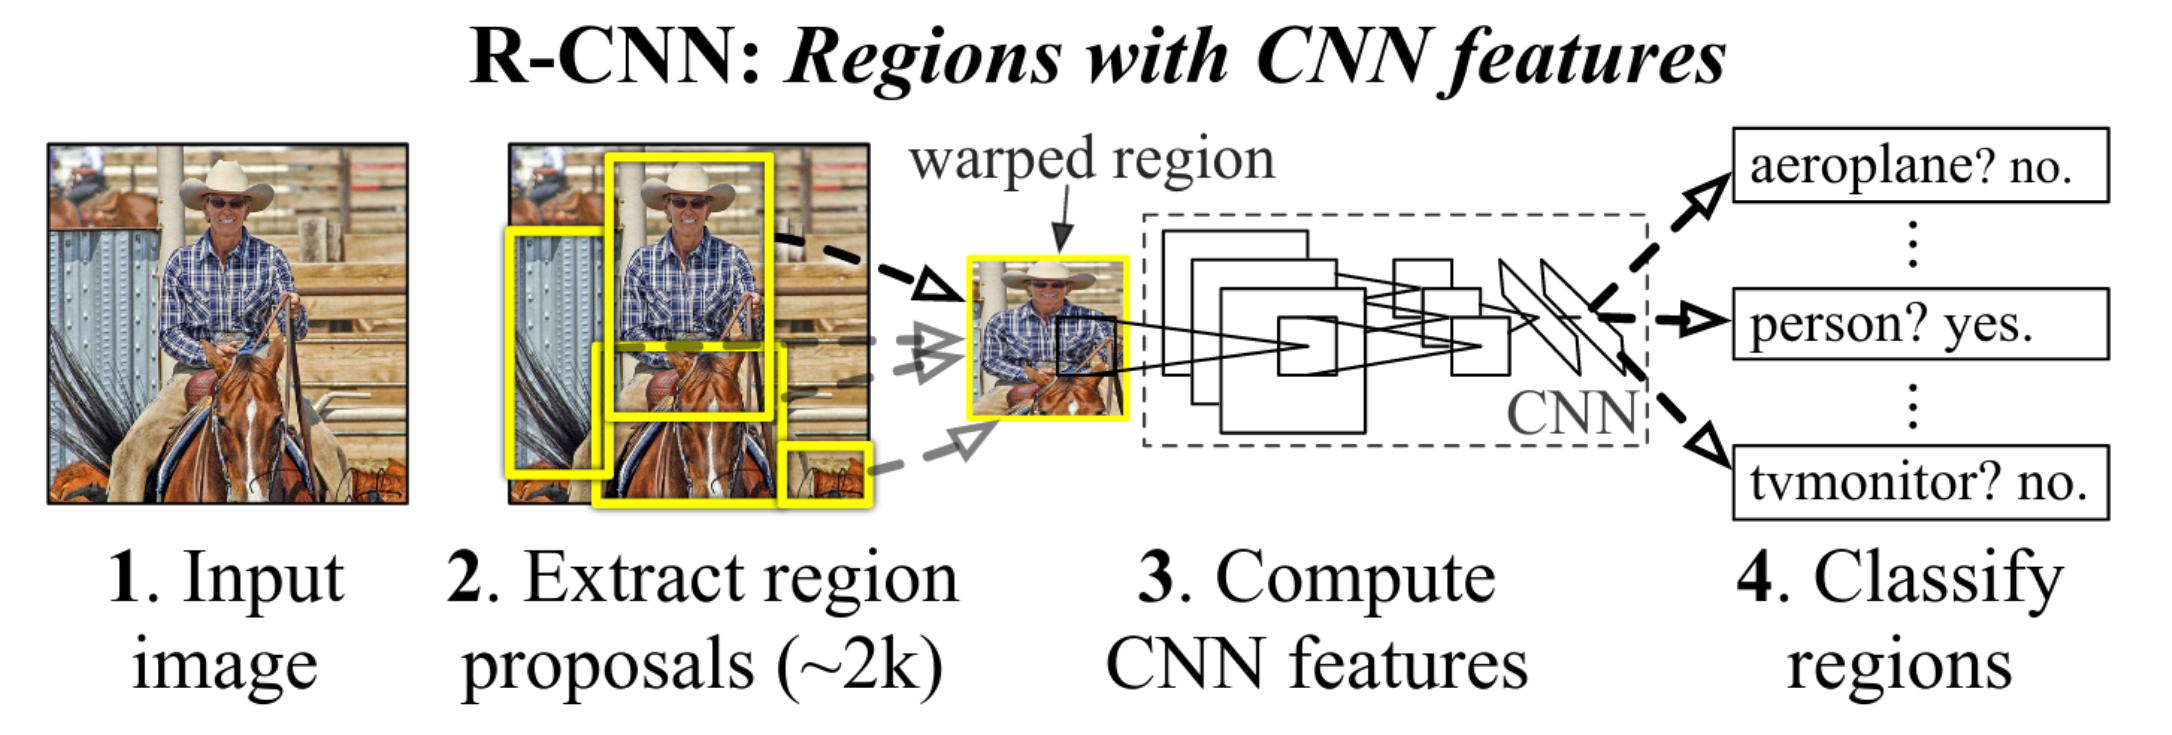
\includegraphics[width=0.9\textwidth]{rcnn}
  \end{figure}

  \note{
    \begin{itemize}
      \item Same author as DPM.
      \item Sliding window as in DPM. But NN much slower as SVM, therefore they used region proposals (2k).
      \item Image from Rich feature hierarchies for accurate object detection and semantic segmentation, Girshick et al, CVPR 2014
    \end{itemize}
  }
\end{frame}


\begin{frame}{Region Proposals}
  \begin{figure}
    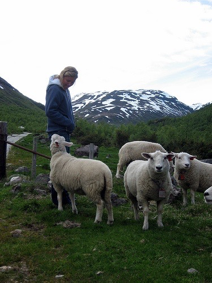
\includegraphics[width=0.15\textwidth]{selective_search_01}
    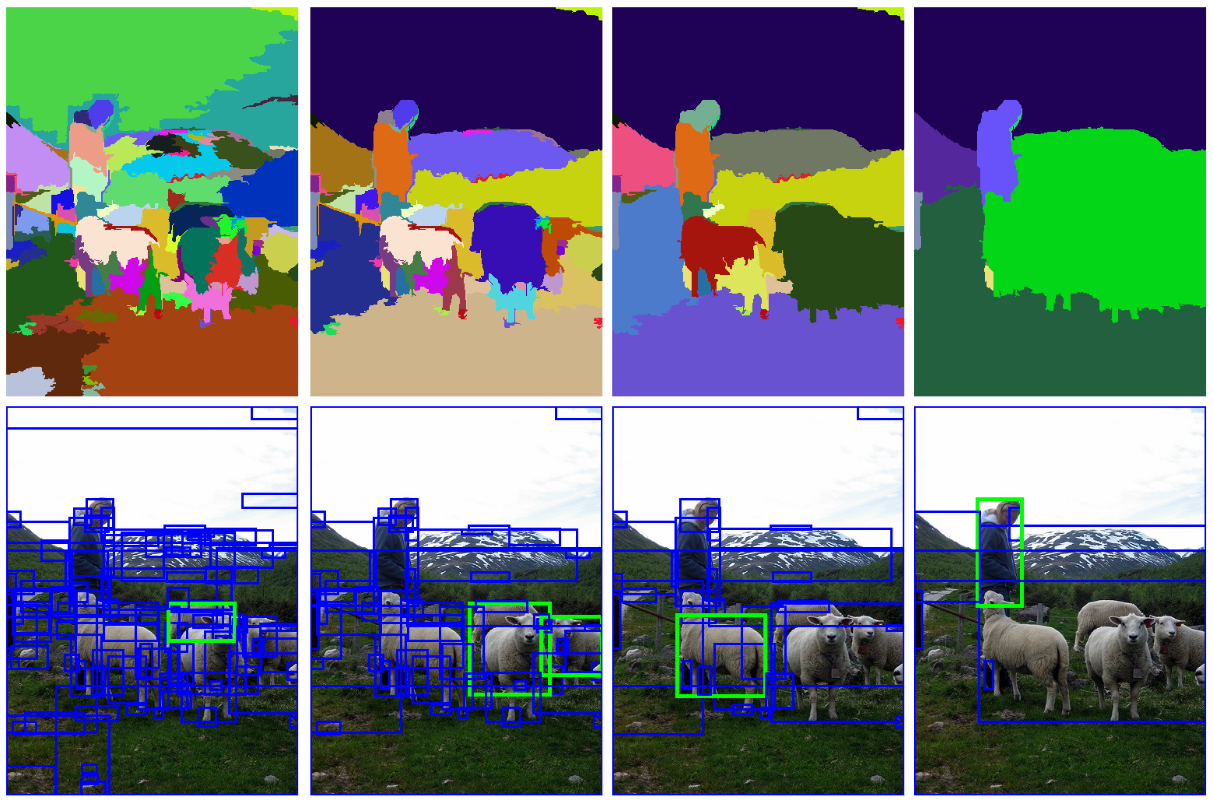
\includegraphics[width=0.65\textwidth]{selective_search_00}
  \end{figure}

  \note{
    \begin{itemize}
      \item Image from Selective Search for Object Recognition, Uijlings et al, IJCV 2013
    \end{itemize}
  }
\end{frame}


\begin{frame}{R-CNN}
  \begin{figure}
    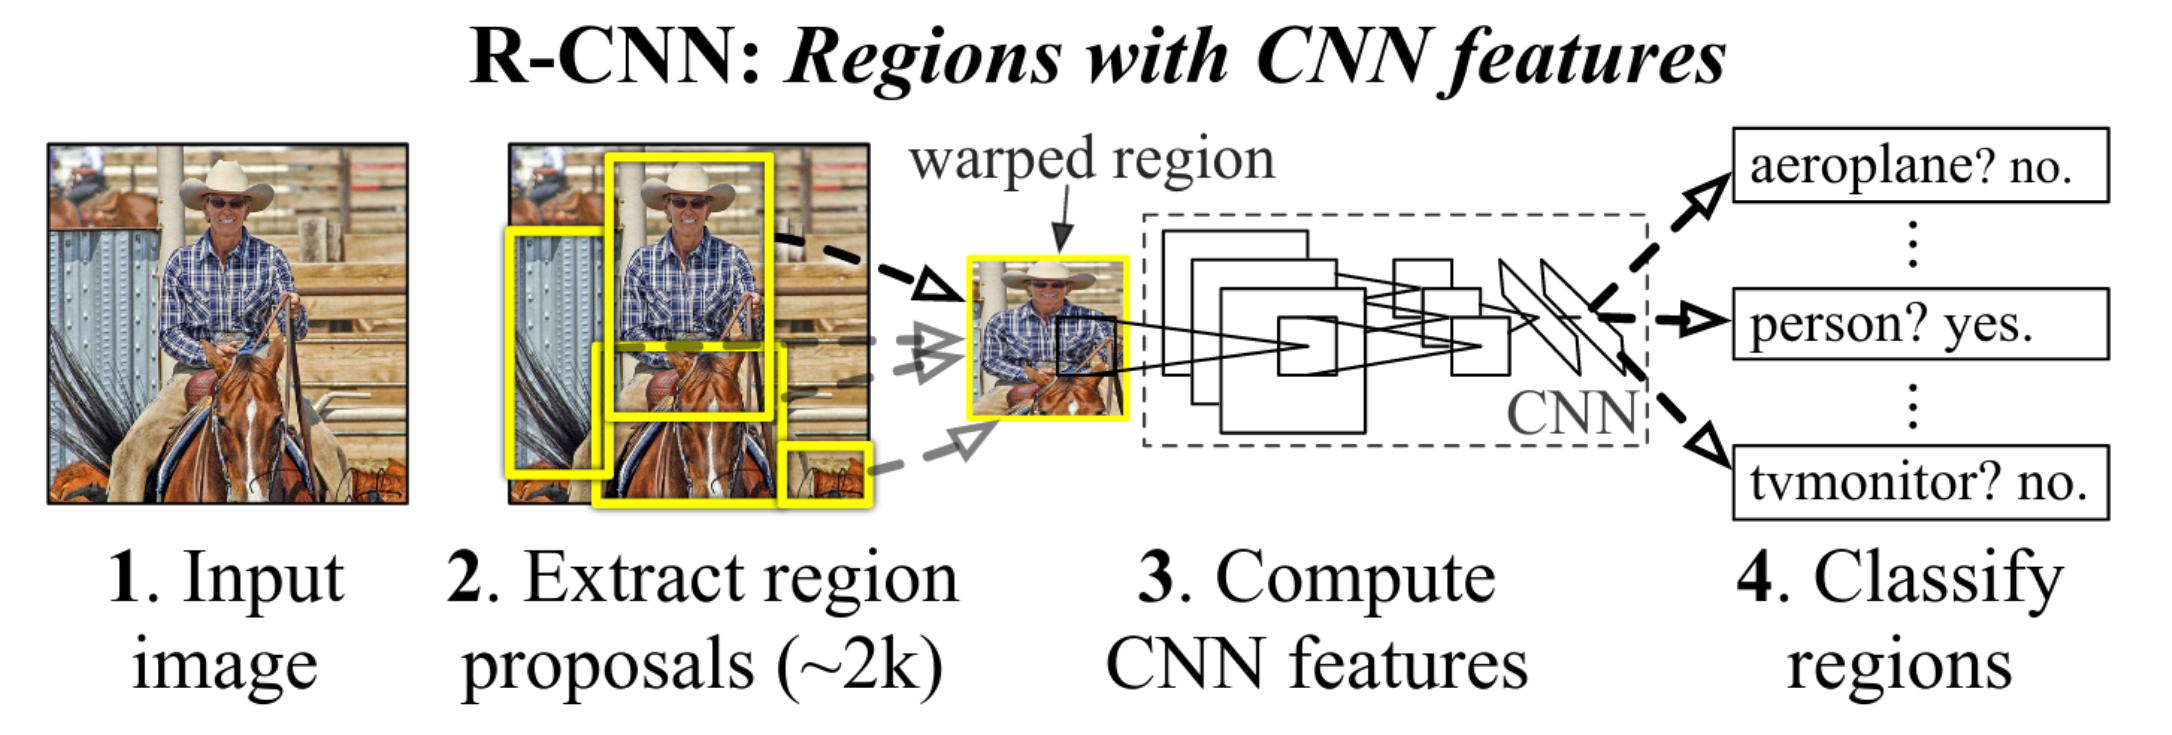
\includegraphics[width=0.9\textwidth]{rcnn}
  \end{figure}

  \note{
    \begin{itemize}
      \item Network also needs to predict bounding box parameters (size and offset from patch center).
      \item Non maximum suppression in prediction space.
      \item Often some high level reasoning (coherence in object relations).
      \item mAP for Pascal VOC improved to 53\% with AlexNet as ConvNet and 62\% with VGG (from 33\% DPM)
      \item Image from Rich feature hierarchies for accurate object detection and semantic segmentation, Girshick et al, CVPR 2014
    \end{itemize}
  }
\end{frame}


\begin{frame}{Fast-RCNN}
  \begin{figure}
    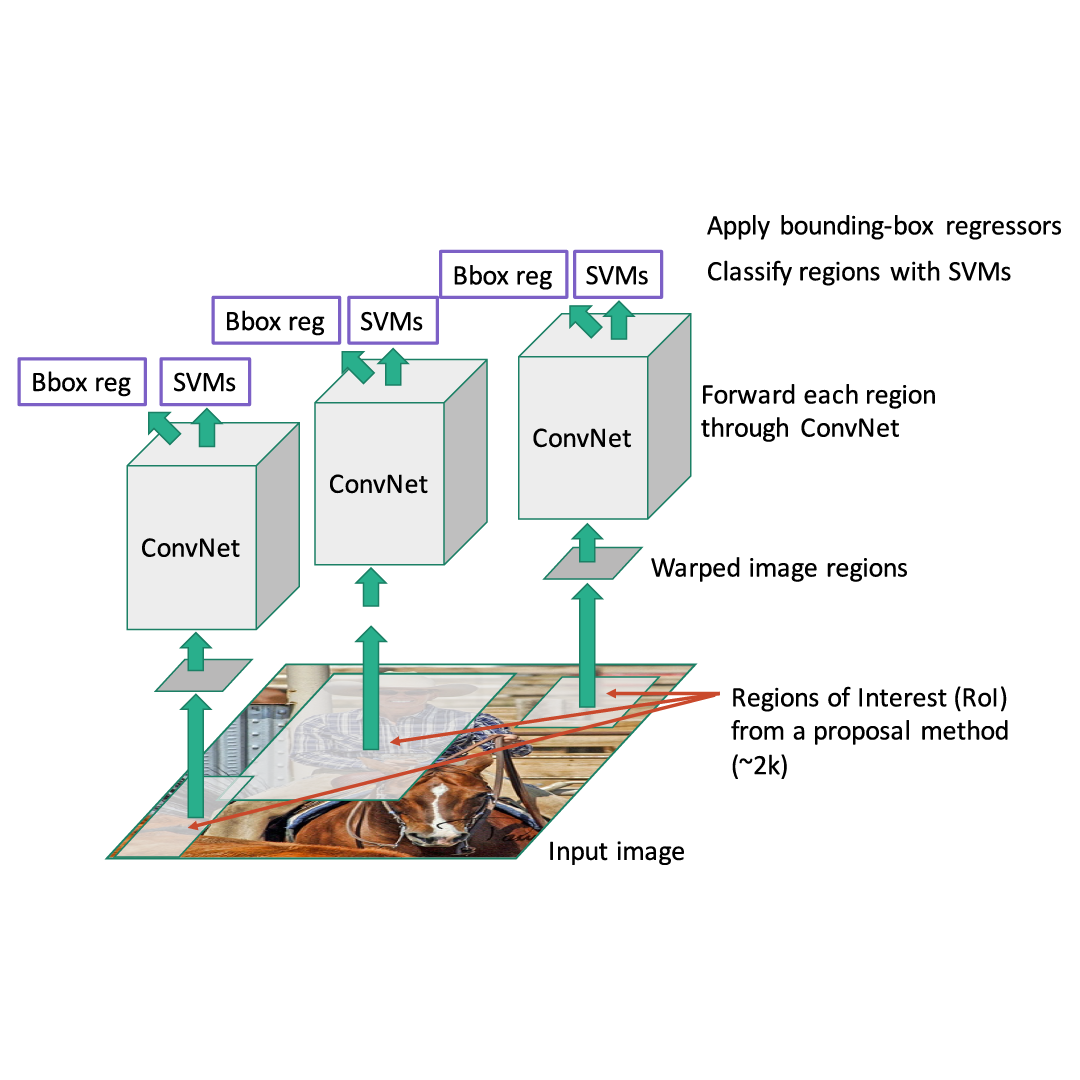
\includegraphics[width=0.45\textwidth]{slow_rcnn}
    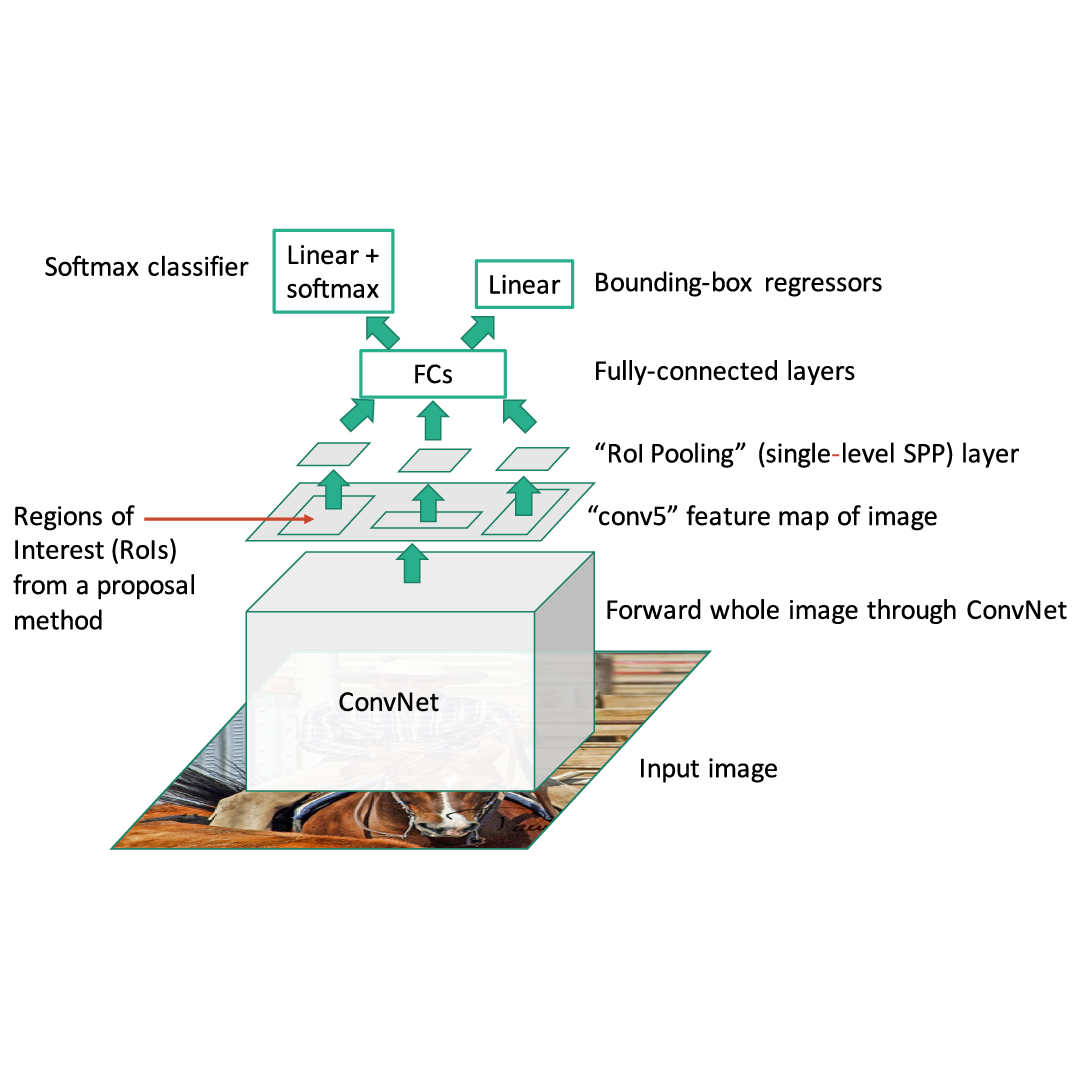
\includegraphics[width=0.45\textwidth]{fast_rcnn}
  \end{figure}

  \note{
    \begin{itemize}
      \item Moves the cropping of proposed regions to the feature map, saving the many forward passes through the convolutional block.
      \item Image from Talk at ICCV 2015 by Ross Girshick \url{https://dl.dropboxusercontent.com/s/vlyrkgd8nz8gy5l/fast-rcnn.pdf?dl=0}
    \end{itemize}
  }
\end{frame}


% \begin{frame}{ROI Pooling}
%   \note{
%     \begin{itemize}
%       \item
%     \end{itemize}
%   }
% \end{frame}


% \begin{frame}{ROI Align}
%   \note{
%     \begin{itemize}
%       \item
%     \end{itemize}
%   }
% \end{frame}



\begin{frame}{Faster-RCNN}
  \begin{figure}
    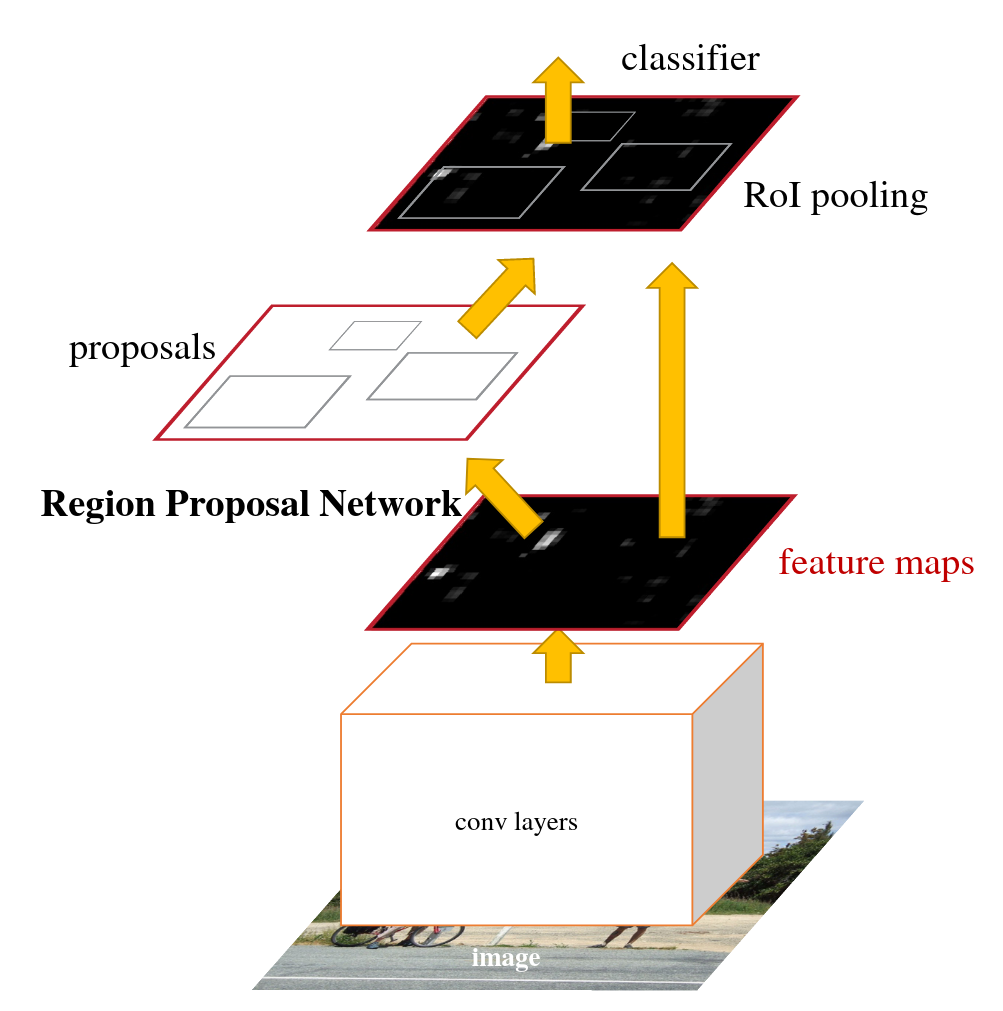
\includegraphics[width=0.5\textwidth]{faster_rcnn}
  \end{figure}

  \note{
    \begin{itemize}
      \item Region proposal is now the expensive step in Fast-RNN.
      \item Faster-RCNN does bounding box regression with a neural network based on the same image features the classifier uses, removing the region proposal step completely.
      \item Solution: Do region proposal in feature map.
    \end{itemize}
  }
\end{frame}


\begin{frame}{YOLO: You Only Look Once}
  \begin{figure}
    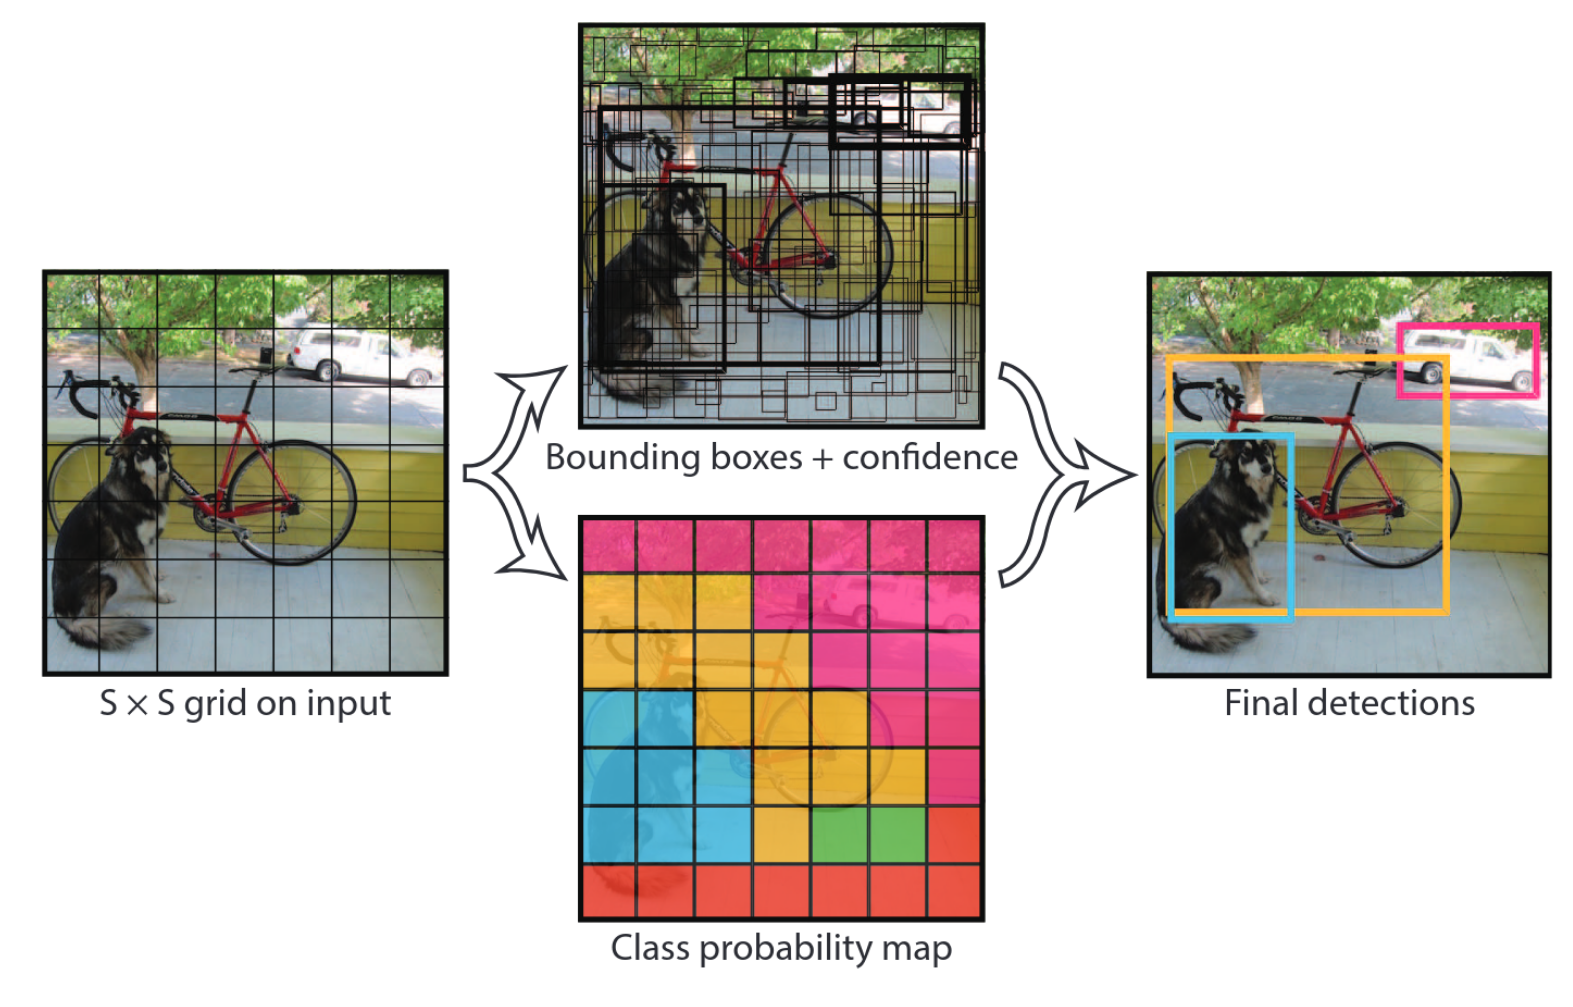
\includegraphics[width=0.8\textwidth]{yolo_00}
  \end{figure}

  \note{
    \begin{itemize}
      \item Image from You Only Look Once:Unified, Real-Time Object Detection, Redmon et al, CVPR 2016
    \end{itemize}
  }
\end{frame}


\begin{frame}{YOLO: You Only Look Once}
  \begin{figure}
    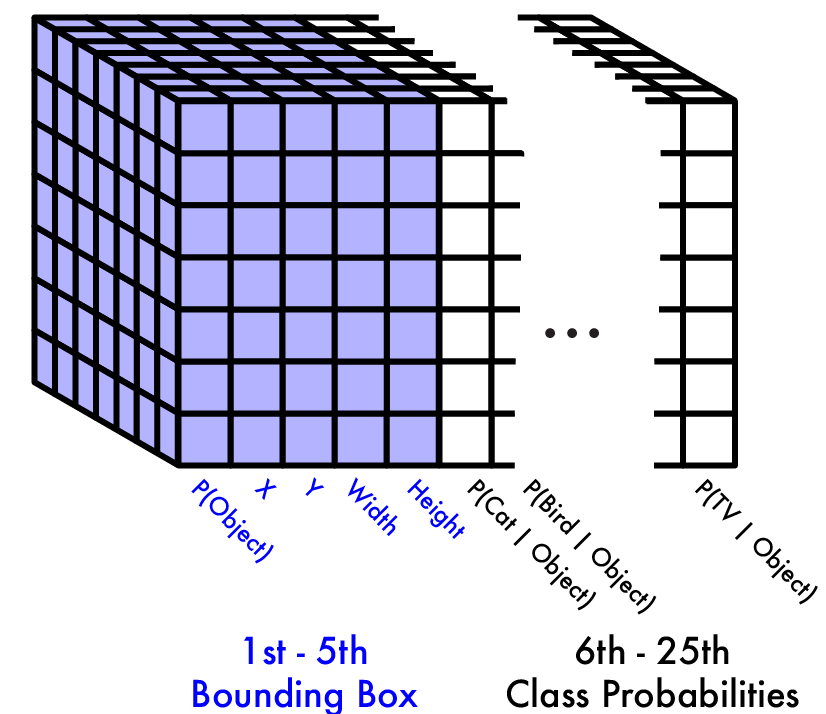
\includegraphics[width=0.55\textwidth]{yolo_01}
  \end{figure}

  \note{
    \begin{itemize}
      \item Newer versions of YOLO have multiple detections per cell for different object sizes.
      \item Image from Ancient Secrets of Computer Vision Lecture 18, Joseph Redmon
    \end{itemize}
  }
\end{frame}



\begin{frame}{YOLO: loss}
  \begin{align*}
    \mathcal{L} &= \alpha_{1}\mathcal{L}_{localization} + \alpha_{2}\mathcal{L}_{object~confidence} + \alpha_{3}\mathcal{L}_{classification} \\
    \mathcal{L}_{localization}&: root~mean~squared~error \\
    \mathcal{L}_{object~confidence}&: binary~cross~entropy \\
    \mathcal{L}_{classification}&: multi-class~cross~entropy
  \end{align*}
  \note{
    \begin{itemize}
      \item weighted loss, binary and multi-class cross entropy, MSE
      \item What would happen without conditional probability?
    \end{itemize}
  }
\end{frame}


% \begin{frame}{RetinaNet}
%   \note{
%     \begin{itemize}
%       \item
%       \item
%     \end{itemize}
%   }
% \end{frame}


\begin{frame}{Why not both? Instance Segmentation}
  \begin{figure}
    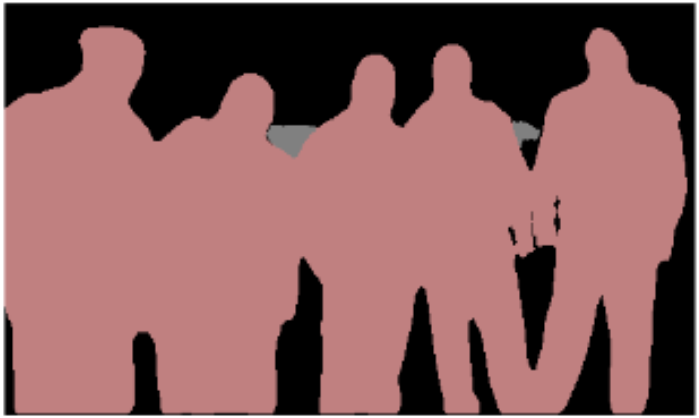
\includegraphics[width=0.5\textwidth]{deeplabv3p_result_person}
    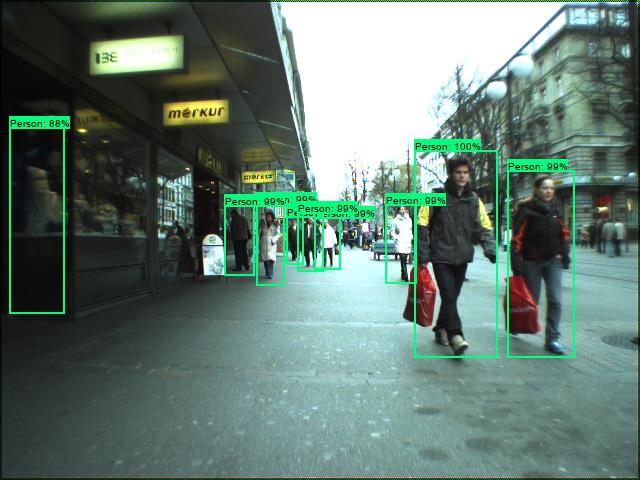
\includegraphics[width=0.4\textwidth]{detection_person}
  \end{figure}

  \note{
    \begin{itemize}
      \item Pixel level classification with instance boundaries.
    \end{itemize}
  }
\end{frame}


\begin{frame}{Mask R-CNN}
  \begin{figure}
    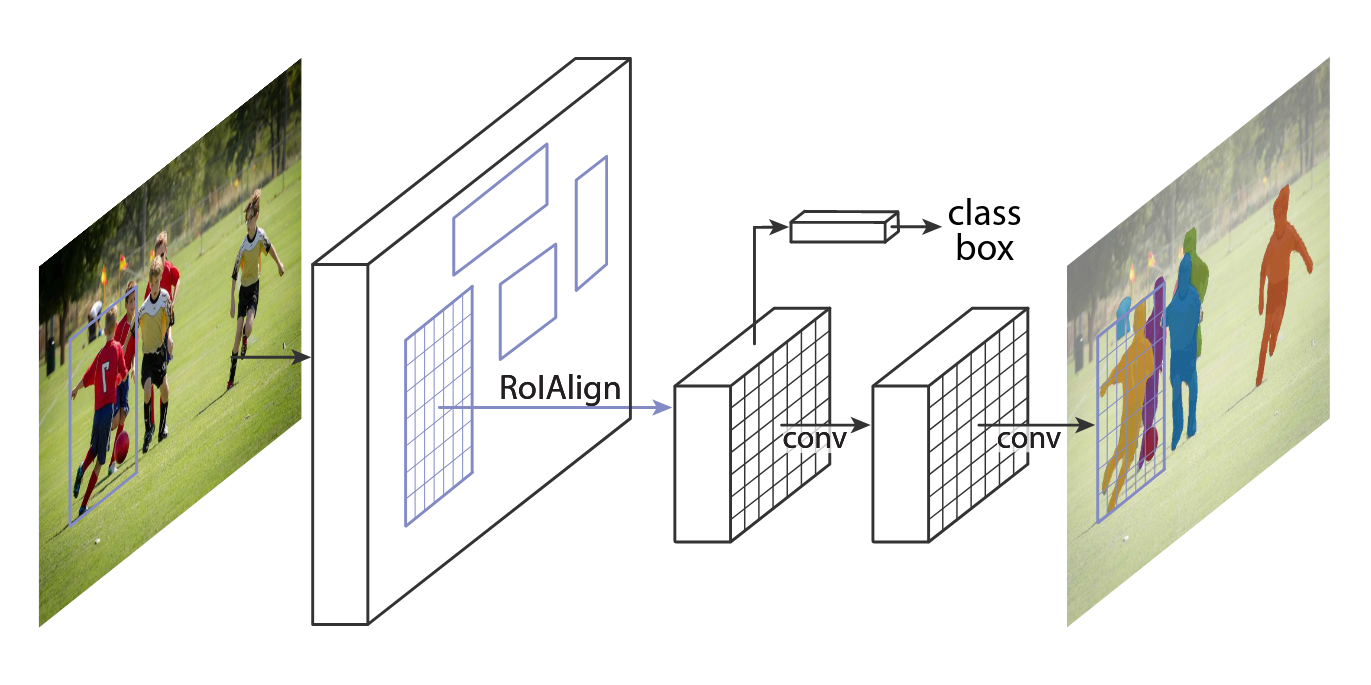
\includegraphics[width=0.9\textwidth]{mask_rcnn}
  \end{figure}

  \note{
    \begin{itemize}
      \item Faster R-CNN with segmentation network.
      \item Image from Mask R-CNN, He et al, ICCV 2017
    \end{itemize}
  }
\end{frame}


\begin{frame}{Mask R-CNN}
  \begin{figure}
    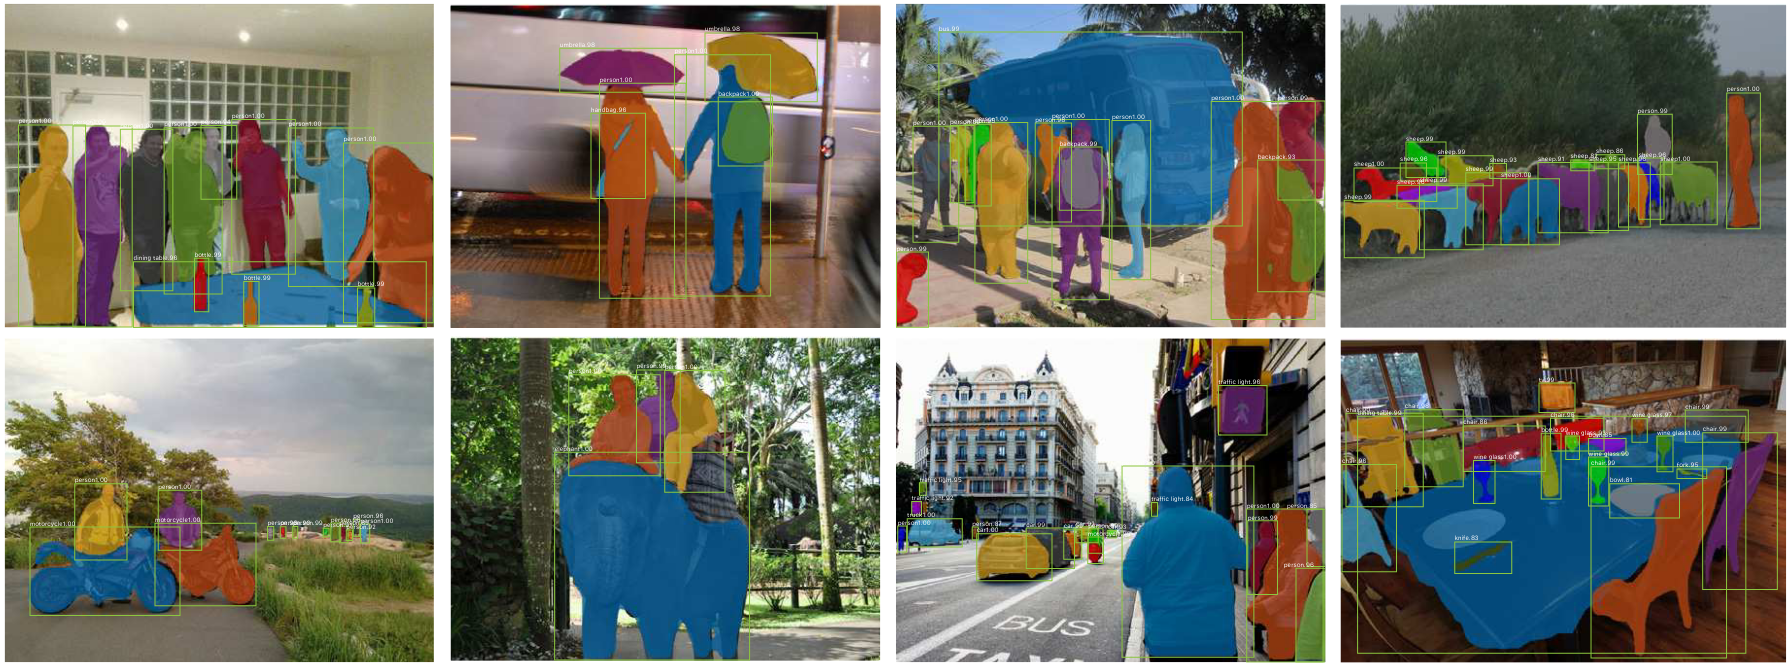
\includegraphics[width=0.9\textwidth]{mask_rcnn_results}
  \end{figure}

  \note{
    \begin{itemize}
      \item Results for Mask R-CNN.
      \item Image from Mask R-CNN, He et al, ICCV 2017
    \end{itemize}
  }
\end{frame}


\begin{frame}{Mask R-CNN}
  \begin{figure}
    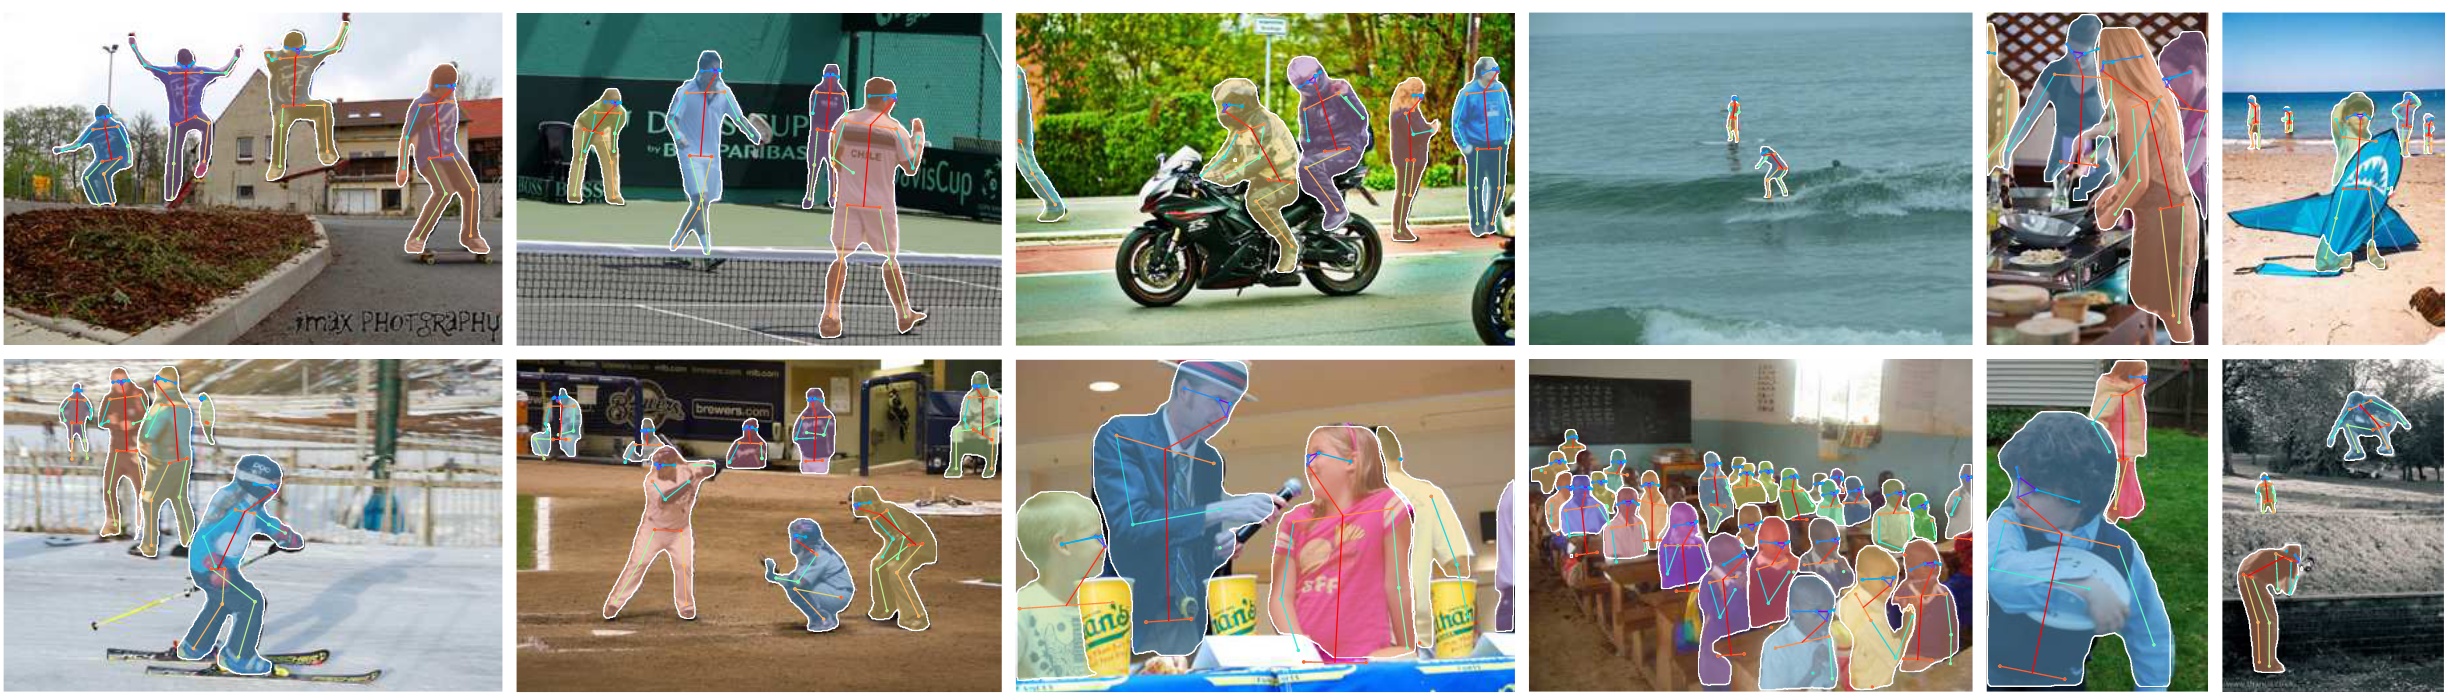
\includegraphics[width=0.9\textwidth]{mask_rcnn_keypoints}
  \end{figure}

  \note{
    \begin{itemize}
      \item Mask R-CNN can also learn skeletons.
      \item Image from Mask R-CNN, He et al, ICCV 2017
    \end{itemize}
  }
\end{frame}
